\section{További vizsgált szempontok - Technológia}
A fent bemutatott esettanulmány csak egy felülnézeti betekintést enged meg nekünk, így szükségesnek tartom kicsit közelebbről is megvizsgálni egy hasonló rendszer bevezetésének technológiai és szervezeti követelményét. Az EMS rendszer képes beavatkozni a gépek működési paramétereibe, ezért közvetlen anyagi károkat okozhat egy szándékosan, vagy véletlenül rosszul beállított gép. Ezen felül az egész rendszer üzemeltetése, karbantartása további kérdéseket vet fel.

\subsection*{Kibertámadások}
A kibertámadások az egyik módja annak, hogy nem megfelelő paraméterek kerüljenek a gyártásba. Mivel a legacy PLC-k és ipari rendszerek nincsenek és nem is lehetnek megfelelően védve a legmodernebb standardok szerint, ezért egy erre szakosodott rendszert kell alkalmazni az effajta kockázatok csökkentésére. Az IEC 62443 adhat egy megfelelő támpontot megfelelő biztonságos rendszerre. Ennek az alapja, hogy szétválasztjuk a vállalati gépeket funkció szerint zónákra (IT, OT, MES, stb.) , amik között az átjárást korlátozva megakadályozhatjuk, hogy egy sebezhetőséget kihasználva a támadók az egész belső hálózathoz hozzáférést.

A Henkelnél folyó optimalizálás folyamatára én egy IEC 62443 egy "Zones and Conduit" elven működő IT/OT hálózati szegmentálást látok megvalósíthatónak. Látható volt a megvalósításról szóló dokumentumokban, hogy egy nagyon sokféle vezérlési folyamatot vonnak be egy mindent összefogó ernyő alá. Ez alapján magas a valószínűsége, hogy rendszert is szükséges hozzácsatolni, ami nem fog elégséges védelemmel rendelkezni a jogosulatlan hozzáférés ellen, ezért védelemre van szüksége ez ellen.
\subsection*{Azonosított kibertámadási forgatókönyvek és sérülékenységek} 
\subsubsection*{R1: Belső munkavállaló által elvégzett jogosulatlan paramétermódosítás} 
\textbf{Leírás:} Egy belső operátor vagy karbantartó jogosulatlanul vagy nem jóváhagyott módon módosítja a PLC vezérlőlogikáját vagy a SCADA határértékeket.  \\\textbf{Következmény:} Sérül az ISO 50001 szerinti mérési adatintegritás, torzulnak az energiateljesítmény-mutatók (EnPI), és hibás automatizált korrekciók keletkeznek.
\subsubsection*{R2: IT--OT átjárón (DMZ Conduit) keresztüli ransomware terjedés} 
\textbf{Leírás:} Zsarolóvírus fertőzi meg a vállalati IT hálózatot, és a nem megfelelően szegmentált hálózati csatornákon (conduit) keresztül átterjed a MES/SCADA szerverekre. \\
\textbf{Következmény:} A gyártósorok azonnali leállása, jelentős kieső termelési volumen és potenciális fizikai berendezéskárosodás.
\subsubsection*{R3: Öregedő (Legacy) HMI-k és PLC-k elleni támadás}
\textbf{Leírás:} A csarnokokban működő, frissítésekkel nem rendelkező HMI terminálok vagy nem frissíthető PLC-k kompromittálása ismert sérülékenységek kihasználásával. \\
\textbf{Következmény:} Lateral movement (oldalirányú terjedés) az OT hálózaton belül, folyamatkontroll elvesztése.
\subsubsection*{R4: IIoT szenzorhálózat adatmanipulációja (Spoofing / Man-in-the-Middle)}
\textbf{Leírás:} A IIoT mérési adatok manipulálása a szenzor és a csatorna közötti nem titkosított kommunikáció során. \\
\textbf{Következmény:} Hamis energiafogyasztási adatok betáplálása a gépi tanulási (ML) optimalizációs modellbe, ami túlfűtéshez vagy energiapazarláshoz vezet.


 \begin{table}[h!] \centering \small \vspace{0.2cm} \begin{tabularx}{\textwidth}{lXcccX} \toprule \textbf{ID} & \textbf{Kockázati esemény} & \textbf{P} & \textbf{I} & \textbf{R} & \textbf{Lehetséges kontrollok}\\ 
 \midrule R1 & Belső jogosulatlan módosítás (PLC/SCADA) & 3 & 4 & \textbf{12} & RBAC, MFA, Active Directory OS csoportok, szigorú Audit Trail. \\
 R2 & IT/OT DMZ Ransomware terjedés & 2 & 5 & \textbf{10} & IEC 62443 Zone \& Conduit szegmentáció, Secure Gateway, adatdióda. \\
 R3 & Legacy HMI/PLC sérülékenység & 4 & 4 & \textbf{16} & Passzív NDR felügyelet, hálózati izoláció, Virtual Patching. \\
 R4 & IIoT szenzor mérési adatspoofing & 3 & 3 & \textbf{9} & OPC UA és MQTT over TLS titkosítás, Continuous Controls Monitoring (CCM). \\
 R5 & Külső OEM távoli hozzáférés visszaélés & 2 & 4 & \textbf{8} & JIT (Just-in-Time) hozzáférés, munkamenet-rögzítés, elszigetelt jump host. \\
\bottomrule
\end{tabularx} 
\caption{Kibervédelmi kockázati mátrix a Henkel--AVEVA rendszerben}
\end{table}
A kockázatok kezelésére a Henkel és az AVEVA architektúrájára a következő kontrollokat alkalmazhatjuk: 
\begin{enumerate} 
\item \textbf{Zónák és Csatornák Szigorítása (IEC 62443 FR 5):} Minden adatáramlást a vállalati IT és az OT zónák között ellenőrzött DMZ csatornákon haladtatunk át. A Secure Gateway modul izolálja a megjelenítési felületeket. 
\item \textbf{Identitás-alapú Kerület (Zero Trust \& RBAC):} Az ArchestrA Galaxy szerepköröket Active Directory csoportházirendekhez kötjük. Az adminisztratív beavatkozásokhoz kötelező a többfaktoros hitelesítés (MFA). 
\item \textbf{Kétszintű OT Monitorozás:} 
\begin{itemize} 
\item \emph{Aktív EDR tier:} Aktív végponti védelem a jump hostokon és mérnöki munkaállomásokon. 
\item \emph{Passzív NDR tier:} Non-intrusive hálózati forgalomelemzés a PLC-k és terepi buszok szintjén. 
\end{itemize} 
\item \textbf{ISO 50001 Adatintegritási Védelem:} Konfigurációeltolódás-figyelés (Configuration Drift Detection), amely azonnal riasztást ad, ha egy mérési paraméter eltér az engedélyezett alapállapottól (baseline). 
\end{enumerate}
\subsection*{Hozzáférési szabályok}
Szintén nincs meghatározva, hogy milyen biztonsági szabályzatot követ a rendszer, ami meghatározná, hogy ki, miért, és hogyan férhet hozzá egy adott Zónához, rendszerhez. Hogyan lehet felosztani egy ekkora komplex rendszerben a jogköröket, és ki melyik működési egységért miben felelős?

\begin{figure}
    \centering
    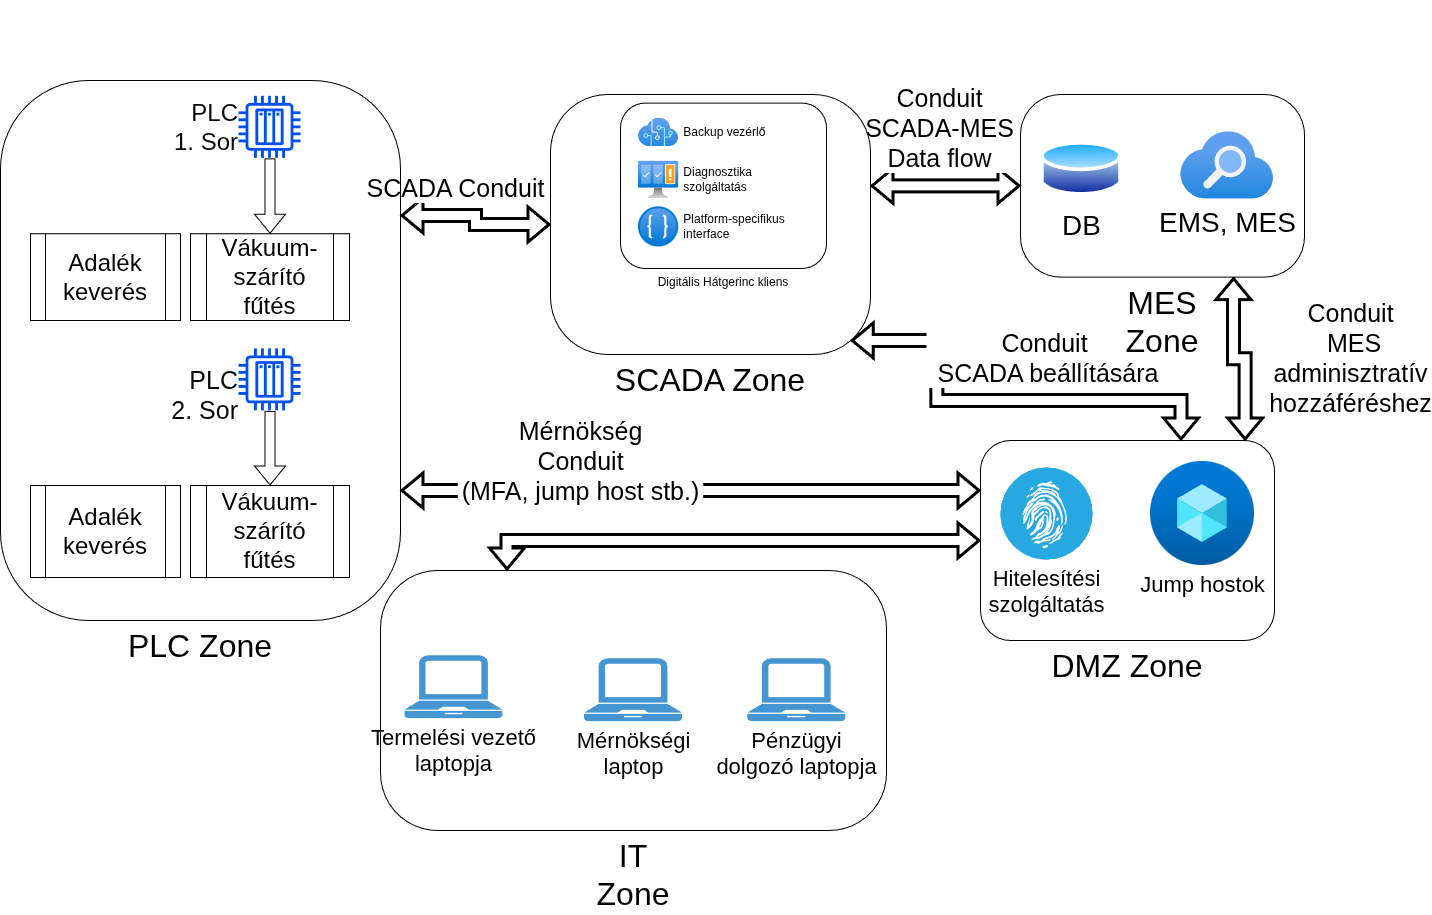
\includegraphics[width=1\linewidth]{images/Z&C.drawio.png}
    \caption{IT/OT Működési zónák működésének vázlata}
    \label{fig:proposal}
\end{figure}
\subsection*{Hibás adatok, adat minőség}
Hogyan észleli, kezeli az automata rendszer, ha valamelyik érzékelő hibás adatokat küld?
Hogy biztosítjuk, hogy a bemeneti adatok hitelesek?
Ez a szempont az ISO 50001 szempontjából is kulcsfontosságú, hiszen az egyik követelménye a szabványnak a hiteles mérési adat, amiből vissza tudjuk ellenőrizni a saját elért energia-megtakarításainkat.

\subsection*{Validáció}
Honnét tudjuk, hogy egy adott 







